\documentclass{beamer}

\usepackage[utf8x]{inputenc}
%\usepackage{default}
\usetheme{Darmstadt}

%\usetheme{Rochester}
%\usetheme{Frankfurt}
%\usetheme{Boadilla}
%\usetheme{Copenhagen}
%\usetheme{Malmoe}
%\usetheme{Pittsburgh}

%\usetheme{Madrid}
%\usetheme{Berkeley}
\usepackage{beamerthemetree}
\usecolortheme{beaver}
\usefonttheme{serif}
%
\title{Monte Carlo Rollout Policy for Recommendation Systems with Dynamic User Behavior}

\author{ \textcolor{blue}{Rahul Meshram (IITM)}  \\
Kesav Kaza (IITB) }
%D.~Manjunath (IIT Bombay)}
\institute{COMSNETS 2021, Bangalore}
\date{ 5th January 2021}
\usepackage{times}
\usepackage{latexsym,graphicx}
%\usepackage{graphicx}
\usepackage{subfigure}
\usepackage{tikz}
\usetikzlibrary{automata,arrows,positioning,calc,decorations.pathreplacing}
%\usepackage{caption}
%\usepackage{subcaption}
%\usepackage[tab]{beamerthemesidebar}
%\usepackage{beamerthemetreebars}
\usepackage{amsmath,amscd,amssymb,amsgen,amsfonts,amsbsy}
\usepackage{algorithmic}
\usepackage[ruled,lined]{algorithm2e}

\beamertemplatenavigationsymbolsempty

\setbeamerfont{page number in head/foot}{size=\large}
\setbeamertemplate{footline}[frame number]

\usepackage{graphicx}
\usepackage[usestackEOL]{stackengine}
\usepackage{xcolor}


\begin{document}

\newcommand{\iid}{{i.i.d.}}
\newcommand{\prob}[1]{\mathsf{Pr}\left( #1 \right)}
%\newcommand{\brac}[1]{\left({#1}\right)}
%\newcommand{\sbrac}[1]{\left[{#1}\right]}
%\newcommand{\cbrac}[1]{\left\{{#1}\right\}}
\newcommand{\remove}[1]{}
\newcommand{\rahul}[1]{\textbf{RAHUL SHOULD FILL THIS/DISCUSS}: \textcolor{blue}{#1}}
\newcommand{\comments}[1]{}
\newcommand{\selfnote}[1]{\textcolor{blue}{\textbf{Note to self:}
    {#1}}}
%\usepackage[english]{babel}
\newcommand{\defn}{{\stackrel{\triangle}{=}}}
%\newcommand{\qed}{\hfill $\square$}
\newcommand{\pd}[2]{\frac{ \partial #1}{\partial #2}}
\newcommand{\md}[2]{\frac{ \partial^2 #1}{\partial #2^2}}
\newcommand{\expect}[1]{\mathsf{E}\left({#1}\right)}
\newcommand{\given}{\; \big\vert \;} 
\newcommand{\bydef}{:=}
\newcommand{\ip}[2]{\langle #1,#2 \rangle}
% Debug
\newcommand{\todo}[1]{\begin{color}{blue}{{\bf~[TODO:~#1]}}\end{color}}



%\newcommand{\EX}{\mathbb{E}} % expectation operator
%\newcommand{\expect}[1]{{\bf E}\left[{#1}\right]}
%\newcommand{\expectpow}[2]{{\bf E}^{#2}\left[{#1}\right]}
%\newcommand{\prob}[1]{\text{Pr}\brac{#1}}
%\newcommand{\pr}{{\cal P}}
%\newtheorem{result}{{\bf Result}}
%\newtheorem{result1}{{}}


\newcommand{\bit}{\begin{itemize}}
\newcommand{\eit}{\end{itemize}}
%\newcommand{\beq}{\begin{equation}}
%\newcommand{\eeq}{\end{equation}}
\newcommand{\beqn}{\[}
\newcommand{\eeqn}{\]}

\newcommand{\eean}{\end{eqnarray*}}
\newcommand{\re}{\mbox{$\mathfrak{Re}$}}
\newcommand{\no}{\nonumber}
\newcommand{\ben}{\begin{enumerate}}
\newcommand{\een}{\end{enumerate}}
\newcommand{\bc}{\begin{center}}
\newcommand{\ec}{\end{center}}

\newcommand{\blem}{\begin{lemma}}
\newcommand{\elem}{\end{lemma}}
\newcommand{\bthm}{\begin{theorem}}
\newcommand{\ethm}{\end{theorem}}
\newcommand{\bdefn}{\begin{definition}}
\newcommand{\edefn}{\end{definition}}
\newcommand{\bpf}{\begin{proof}}
\newcommand{\epf}{\end{proof}}

%%%%%%%%%%%%%%%%%%%%%%%%%%%%%
%%%%%%%%%%%%%%%%%%%%%%%%%%%bracket
\newcommand{\brac}[1]{\left({#1}\right)}
\newcommand{\sbrac}[1]{\left[{#1}\right]}
\newcommand{\cbrac}[1]{\left\{{#1}\right\}}
% \newtheorem{ex}{Example}
%%%%%%%%%%%%%%%%%%%%%%%%%%%%%%%%
\newtheorem{remark}{Remark}
\newtheorem{assumption}{Assumption}

%\newcommand{\expc}[2][]{E^{#1}\left[{#2}\right]}
%\newcommand{\set}[1]{\{#1\}}

%\newcommand{\ul}{\underline}
%\newcommand{\smq}[1]{{\it #1}}
%\newcommand{\ave}[1]{\overline{#1}}

%%%%%%%%%%%%%%%%%%%%
\newlength{\firstimage}
\setlength\firstimage{0.5\paperwidth}
\newlength{\secondimage}
\setlength\secondimage{0.5\paperwidth}

%%%%%%%%%%%%%%%%%%%%%%%%%%%%%%%%%%%5

\def\calloutsym{%
  \ensurestackMath{%
  \scalebox{2}{\color{red}\stackunder[2pt]{}{\downarrow}}}%
}
\newcommand\callouttext[1]{%
  \def\stacktype{S}\renewcommand\useanchorwidth{T}\stackText%
  \stackunder{\calloutsym}{\scriptsize\Longstack{#1}}\stackMath%
}
\newcommand\callout[3][1.5pt]{%
  \def\stacktype{L}\stackMath\stackunder[#1]{#2}{\callouttext{#3}}%
}


%%%%%%%%%%%%%%%%%%%%%%%%%%%%%%%%5
\frame{\titlepage}

\section{Motivation}

%\frame{
%\frametitle{ Playlist generator}
%\begin{columns}
% \begin{column}{0.5 \textwidth}
%   \bit
%     \item<1-> Playlist generator has a list of $N$ items in its database.
%     \item<2-> It plays items sequentially to the user.
%     \item<3-> The user provides a binary feedback, e.g.,  clicking on 
%``like'' 
%%or ``dislike''
% button.
%\item<3-> Example: Pandora internet radio.
%     \item<4-> The user’s interest in an  item  is determined by 
%       {
%         \bit
%           \item<4-> intrinsic interest 
%           \item<4-> time since it was last played.
%          \eit%
%         % Need a figure
%       }
%     \eit
% \end{column}
%
% \begin{column}{0.5\textwidth}
%%\bit
%%\item<3->
%   \begin{figure}
%     \begin{center}
%    %   \begin{tabular}{cccc}
%         \includegraphics[scale=0.24]{music-rs.png}  
%    %   \end{tabular}
%     \end{center}
%   \end{figure}
%%\eit
% \end{column}
%\end{columns}
%}
%------------------

\frame{ 
\frametitle{Motivation}
\bit 
\item User visits to a recommendation system (RS)
\item RS recommends item sequentially to the user
\item The user provides feedback based on his interest.  
\item Recommendation systems examples---Netflix, Amazon Prime, Spotify, Youtube, etc.
\item Recommendation system generates personalized playlists. 
\item The playlist is generated using information from watch history or information from social networking sites.  	
\eit 	
}

\frame{ 
\frametitle{Recommendation systems models}
\bit 
\item Collaborative filtering approach: 
\item Matrix completion method for RS:
\item \textcolor{blue}{In these models: it is implicitly assumed that the user interest is static and the current recommendation does not influence future behavior of  user interest.}
\item \textcolor{red}{Our model: We assume that user behavior is dynamic, i.e., the user interest is influenced by current recommendation as well as preceding recommendations. } 
\item We consider Markov model for user interest, a state describes the intensity level of preferences.
\item Objective: Model and analyze the dynamic playlist generation systems using binary feedback from user 
\eit 
 	
}

\frame{ 
\frametitle{Our model assumptions}
\bit 
\item There are $N$ independent items 
\item There are different items, the user state for different items will be different
\item State of the user interests for items is not observable
\item Belief about the state is maitained by RS
\item State evolution for each item is different and this evolution depends on whether item played or not 
\item Only one item is played to the user at a time
\item Each item can be modeled as partially observable Markov decision process (POMDP)
\item RS has many items and these are weakly coupled since only one item is allowed to play
%\item Goal is to determine sequence in which items to play to maximize long term reward


\eit 	
	
}

\frame{
	\frametitle{Connection to Restless multi-armed  bandit }
	%\begin{onlyenv}<1>
	%Restless bandit:
	
	\begin{columns}
		\begin{column}{0.67\textwidth}
			\bit
			\item<1-> There are $N$ independent arms.
			\item<1-> Each arm can be in  one of  many  states.
			\item<1-> At each time step,   one arm is played.
			\item<1-> Playing  of arm yields a unit  reward that depends on the state of that arm. 
			\item<1-> State of each  arm  evolves at every time step. 
			\item<1-> This evolution depends on whether an arm is played or not.
			\item<1-> \alert{Goal: Determine  sequence of arms to play  that  maximizes
				a  long run  reward function.}
			
			%\item<6-> Each arm is modeled as MDP/POMDP with two actions.
			
			\eit 
		\end{column}
		%
		\begin{column}{0.3\textwidth}
			\begin{figure}
				\begin{center}
					%   \begin{tabular}{cccc}
					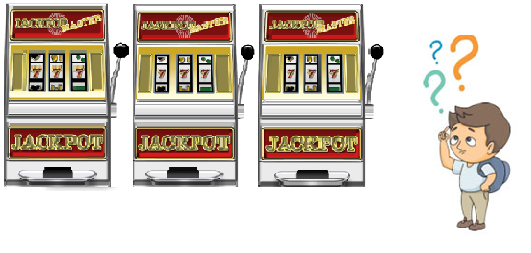
\includegraphics[scale=0.3]{rmab.png}  
					%   \end{tabular}
				\end{center}
			\end{figure}
		\end{column}
	\end{columns}
	
}

\frame{ 
\frametitle{Solution Approach} 	
\bit 
\item RMAB is PSPACE complete problem. Hence the optimal solution is difficult.
\item Popular heuristic policies are 
{
\bit  
\item Myopic policy: Play item with highest immediate expected payoff
\item Whittle index policy \cite{Whittle88}: Play item with highest index, the index is mapping from state to a real number
{
	\bit 
	\item  Difficulty: Need to show indexability and obtain closed form expression for  index in terms of state and rewards
	\item In general, no closed form solution for index with  POMDP model
	\item Literature: \cite{Meshram17a}, specialized model is studied with two state POMDP, special structure is assumed, and index formula is derived
	\eit 
}
\item Our approach:  Monte Carlo rollout policy
{
\bit 	
\item This is simulation based approach for complex problem
\item No structural assumption is made
\item Recent literature \cite{Meshram2020}, \cite{Bertsekas20}, \cite{Bertsekas20b}
%\item Other application of this 
\eit 
}

\eit 
}

\eit 	
}

\frame{ 
\frametitle{Monte Carlo rollout policy} 

\bit 
\item  $L$ trajectories are simulated for a fixed horizon length $H$ using a fixed policy $\phi$   
\item The  information obtained from a single trajectory is
%\begin{eqnarray*} 
$\{ \pi_{j,t,l},a_{j,t,l}, R_{j,t,l}^{\phi}\}_{j=1,t=1}^{ N,  H}$
%\end{eqnarray*} 
%under policy $\phi.$
%\item The value estimate of  trajectory $l$ starting from belief state $\pi$ for $N$ items and initial action $a$    
%\begin{eqnarray*}
%	Q_{H,l}^{\phi}(\pi, a) = \sum_{h=1}^{H} \beta^{h-1} R_{h,l}^{\phi} 
%= \sum_{h=1}^{H} \beta^{h-1} r(\pi_{h,l},a_{h,l}, \phi).
%\end{eqnarray*}  
\item Then, the value estimate for state $\pi$ and action $a$ over $L$ trajectories under policy $\phi$ is 
\begin{eqnarray*}
	\widetilde{Q}_{H,L}^{\phi}(\pi, a) = \frac{1}{L}\sum_{l=1}^{L}    Q_{H,l}^{\phi}(\pi, a, W) = \frac{1}{L}\sum_{l=1}^{L} \left[\sum_{h=1}^{H} \beta^{h-1} r(\pi_{h,l},a_{h,l}, \phi) \right]
\end{eqnarray*} 
\item  A one step policy improvement is performed, and the optimal action  is selected according follow rule. 

\begin{eqnarray*}
j^*(\pi) = \arg \max_{1 \leq j \leq N} \left[ r(\pi, a= j) + \beta \widetilde{Q}_{H,L}^{\phi}(\pi, a = j) \right].
\end{eqnarray*}	
\eit 	
}


%-------------------
\frame{
\frametitle{Numerical Examples} 
\begin{onlyenv}<1>
	
	\begin{figure}
		\begin{center}
			\begin{tabular}{cccc}
%				\includegraphics[scale=0.35]{1_N10.pdf}
				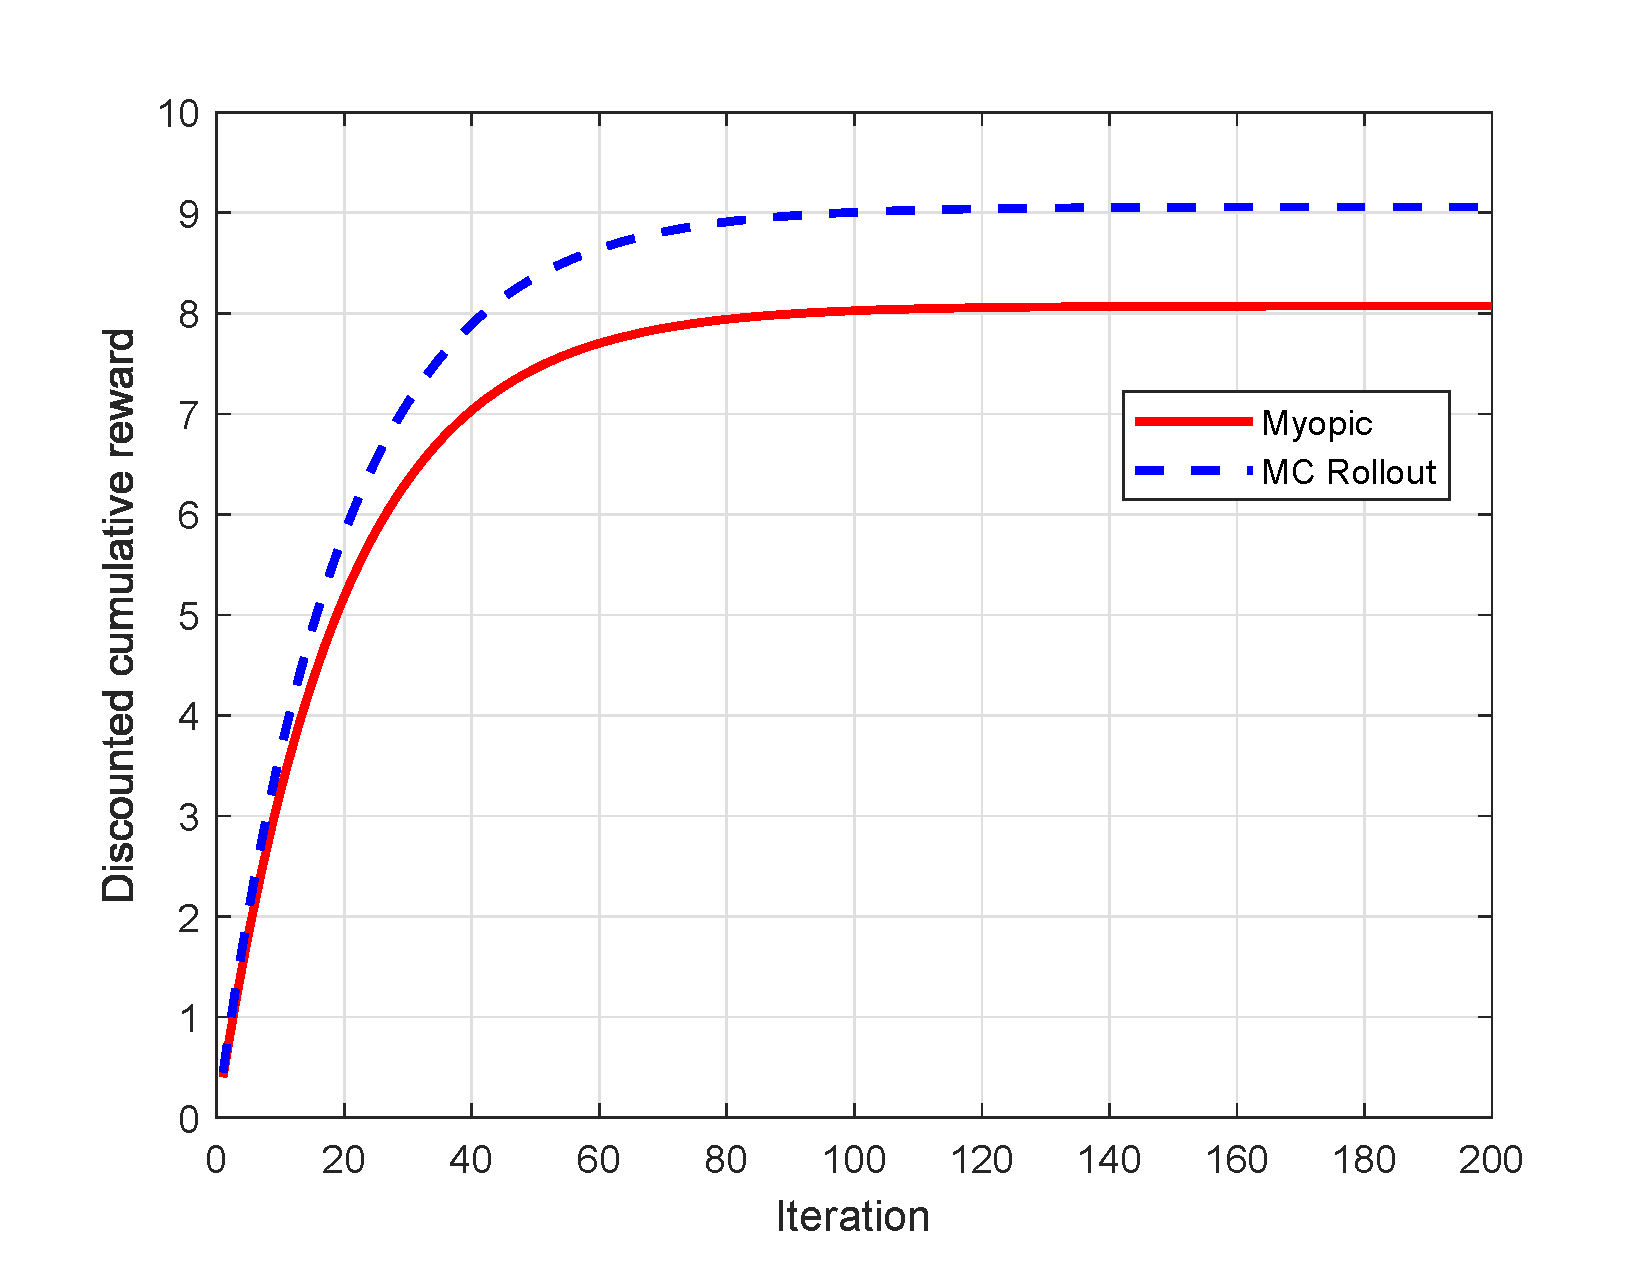
\includegraphics[scale=0.2]{Myopic_MCpolicyEx3.pdf}
				& 
				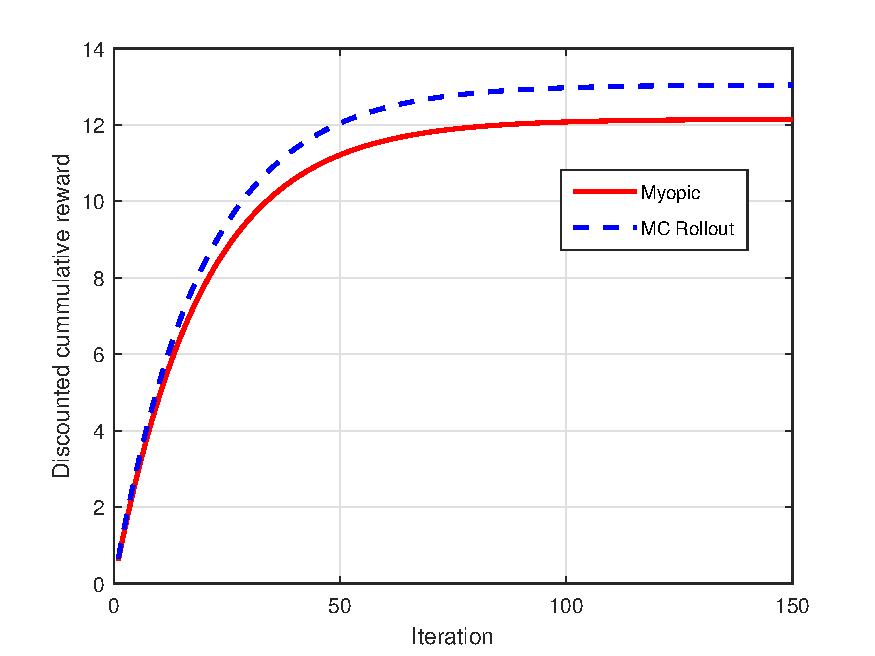
\includegraphics[scale=0.38]{MC_MP_15arms2.pdf} \\
				%\includegraphics[scale=0.35]{1_N200.pdf} \\
				a) $N=5$  & b) $N = 15$
			\end{tabular}
		\end{center}
		%\caption{Cumulative reward vs time horizon for different $N.$  }
		\label{Fig-CR-2}
	\end{figure}
	
	\alert{\em{Remark}}
	\bit
	\item  Monte Carlo rollout policy performs better than myopic
	\item  No structural assumption on transition dynamics is assumed
	%\item Because large $N,$ waiting time for each item is large and 
	%that may result to many items being in state $1$ with high probability. 
	\eit 
\end{onlyenv}


}


\frame{ 
\frametitle{Concluding remarks and future work} 
\bit 
\item Concluding remarks: 
{
\bit 	
\item  We presented a new Monte
Carlo rollout algorithm for RS with Markov model. 
\item We  demonstrated the performance of the
algorithm on a small scale example.
\item We observed that Monte Carlo rollout policy performs better for
arbitrary transition dynamics
\eit 
}
\item Future work:
{
\bit 
\item How to design RS  assuming there is cognitive limitation of human and information overload problem

\item Modeling of user dynamic behavior using other models (Non Markovian) which can characterize complex behavior of user.  
\eit 
}
\eit 

}


\section{Bibliography}
\begin{frame}[allowframebreaks]
\frametitle{Bibliography}
\footnotesize
% \fontsize{6pt}{7.2}\selectfont
\bibliographystyle{apalike}
\bibliography{restless-bandits.bib}
\end{frame}


\end{document}